% FAIR'2026 — Springer LNCS template (XeLaTeX, tiếng Việt)
% Finalized submission-ready manuscript.
% Compile: ./compile.sh
%
% RESULT PLACEHOLDERS: every empirical number is wrapped in \ph{...}. After
% re-running the (leakage-free) pipeline, replace each \ph{...} with the value
% from the corresponding results/*.csv. Do NOT reuse the legacy F1=1.000
% numbers — they came from a configuration with destination_port leakage and
% feature-level duplicate flows, both now removed.
%
\documentclass[runningheads]{llncs}

\usepackage{fontspec}
\usepackage{polyglossia}
\setdefaultlanguage{vietnamese}
\setotherlanguage{english}
% Shared XeLaTeX font setup for Vietnamese manuscripts.
% TeX Gyre Termes is a Times-compatible font that ships with TeX Live / MacTeX,
% covers Vietnamese, and needs no MS-Office fonts -> builds on any machine.
% If you have "Times New Roman" installed and your venue requires it exactly,
% swap the line below for: \setmainfont{Times New Roman}[Ligatures=TeX]
\setmainfont{TeX Gyre Termes}[Ligatures=TeX]

\usepackage{graphicx}
\usepackage{booktabs}
\usepackage{multirow}
\usepackage{amsmath}
\usepackage{xcolor}
% babel defines \babelshorthandoff; under polyglossia it is undefined, so
% provide a no-op fallback to avoid an "Undefined control sequence" at
% \begin{document} (Vietnamese shorthands are not active under polyglossia).
\providecommand{\babelshorthandoff}[1]{}
\AtBeginDocument{\babelshorthandoff{"}\babelshorthandoff{'}}

% Visible placeholder for a not-yet-filled empirical value.
\newcommand{\ph}[1]{{\color{red}\textbf{[#1]}}}

\graphicspath{{../../../results/ml_07_cross_method_comparison/}{../../../results/ml_05_shap_explainability/}{../../../results/ml_09_multiclass_eval/}{../../../results/ml_10_leakage_ablation/}}

\begin{document}

\title{So sánh giảm chiều và lựa chọn đặc trưng cho phát hiện xâm nhập mạng trên Apache Spark ML với quy trình đánh giá chống rò rỉ}

\titlerunning{Giảm chiều và lựa chọn đặc trưng cho IDS trên Spark}

\author{Nguyễn Vũ Thái\inst{1} \and Bùi Văn Dũng\inst{2,3}}
\authorrunning{N. V. Thái et al.}
\institute{Trường Đại học Giao thông Vận tải, Phân hiệu tại TP. Hồ Chí Minh, Việt Nam\\
\email{nvthai@utc2.edu.vn}
\and
Đại học Quốc gia TP. Hồ Chí Minh, Việt Nam
\and
Trường Đại học Công nghệ Thông tin, Việt Nam\\
\email{dungbv.17@grad.uit.edu.vn}}

\maketitle

\begin{abstract}
Hệ thống phát hiện xâm nhập mạng (IDS) dựa trên học máy thường xử lý hàng trăm đặc trưng luồng mạng, gây tốn kém tính toán và khó triển khai tại biên. Bài báo trình bày một nghiên cứu so sánh có hệ thống bốn chiến lược giảm chiều trên Apache Spark ML --- baseline toàn bộ đặc trưng, lựa chọn theo Random Forest Importance, lựa chọn theo SHAP, và PCA --- trên tám thuật toán phân loại cùng hai phương pháp ensemble, đánh giá trên tập CICIDS2017~\cite{sharafaldin2018toward}. Khác với phần lớn công trình trước, chúng tôi nhấn mạnh \emph{tính nghiêm ngặt của quy trình đánh giá}: (i) loại đặc trưng rò rỉ nhãn \texttt{destination\_port} và khử các luồng trùng lặp ở mức đặc trưng trước khi chia dữ liệu; (ii) cố định cấu hình so sánh \emph{a priori} để tránh thiên lệch chọn lọc; (iii) đánh giá robustness trên holdout \emph{tách rời hoàn toàn} khỏi tập huấn luyện; (iv) kiểm định ý nghĩa thống kê bằng permutation test ghép cặp trên nhiều lần lấy mẫu lại dữ liệu; và (v) bổ sung đánh giá đa lớp theo từng loại tấn công. Kết quả cho thấy lựa chọn đặc trưng giữ được phần lớn hiệu năng phân loại trong khi giảm khoảng 60\% số đặc trưng; SHAP Top-30 cân bằng giữa độ chính xác, khả năng giải thích và chi phí, phù hợp để export sang thiết bị biên Jetson Orin Nano Super (xem công trình liên quan).

\keywords{Phát hiện xâm nhập \and Apache Spark \and Lựa chọn đặc trưng \and SHAP \and Rò rỉ dữ liệu \and CICIDS2017.}
\end{abstract}

\section{Giới thiệu}
\label{sec:intro}

Tấn công mạng ngày càng gia tăng về quy mô và độ tinh vi, đòi hỏi các hệ thống IDS vừa chính xác vừa mở rộng được trên dữ liệu lớn~\cite{ring2019survey,khraisat2019survey}. Học máy đã trở thành hướng chủ đạo cho IDS dựa trên bất thường, nhưng các bộ dữ liệu luồng mạng hiện đại như CICIDS2017~\cite{sharafaldin2018toward} cung cấp gần 80 đặc trưng mỗi luồng, làm tăng chi phí huấn luyện, suy luận và bộ nhớ --- đặc biệt nghiêm trọng khi triển khai tại biên. Giảm chiều và lựa chọn đặc trưng vì vậy là bước then chốt, song các chiến lược khác nhau (embedded, không giám sát, dựa trên giải thích) đo ``mức quan trọng'' theo những cách không tương đương và hiếm khi được so sánh trên cùng một pipeline phân tán.

Một vấn đề ít được chú ý nhưng nghiêm trọng không kém là \emph{độ tin cậy của quy trình đánh giá}. Nhiều báo cáo trên CICIDS2017 đạt F1 xấp xỉ tuyệt đối ở bài toán nhị phân; điều này thường là dấu hiệu rò rỉ dữ liệu hơn là năng lực mô hình. Hai nguồn rò rỉ phổ biến: (1) đặc trưng \texttt{destination\_port} mã hoá trực tiếp dịch vụ bị tấn công (CICIDS2017 sinh các kịch bản tấn công nhằm vào cổng cố định), trở thành ``lối tắt'' ghi nhớ ánh xạ cổng~$\rightarrow$~nhãn; và (2) các luồng trùng lặp ở mức đặc trưng không bị loại bởi khử trùng tuyệt đối, khiến phép chia ngẫu nhiên đặt cùng một mẫu vào cả train lẫn test. Bài báo xử lý cả hai trước khi so sánh phương pháp.

\textbf{Đóng góp chính.}
(1) So sánh đồng nhất RF Importance, SHAP và PCA trên cùng tám thuật toán Spark ML và hai ensemble;
(2) Tích hợp giải thích bằng SHAP~\cite{lundberg2017unified} và đối chiếu trực tiếp với RF Importance~\cite{breiman2001random};
(3) Một quy trình đánh giá \emph{chống rò rỉ và có kiểm định thống kê}: loại đặc trưng rò rỉ, khử trùng mức đặc trưng, robustness trên holdout tách rời, permutation test ghép cặp trên nhiều lần lấy mẫu lại;
(4) Đánh giá đa lớp theo từng loại tấn công, làm rõ nơi các phương pháp thực sự khác biệt;
(5) Khuyến nghị lựa chọn mô hình \emph{edge-aware} (F1, số đặc trưng, kích thước) cho Jetson Orin Nano Super.

Phần~\ref{sec:related} trình bày nghiên cứu liên quan; Phần~\ref{sec:method} mô tả phương pháp và quy trình đánh giá; Phần~\ref{sec:exp} báo cáo thí nghiệm; Phần~\ref{sec:discuss} thảo luận; Phần~\ref{sec:threats} nêu các mối đe doạ đến tính hợp lệ; Phần~\ref{sec:conclude} kết luận.

\section{Nghiên cứu liên quan}
\label{sec:related}

Các khảo sát IDS~\cite{ring2019survey,khraisat2019survey,ferrag2020deep} cho thấy cả học máy truyền thống lẫn học sâu được áp dụng rộng rãi trên các bộ chuẩn như CICIDS2017~\cite{sharafaldin2018toward}. Nhiều công trình tập trung một thuật toán đơn lẻ --- Random Forest trực tuyến~\cite{alrawashdeh2016toward} hoặc mạng sâu~\cite{vinayakumar2019deep} --- mà chưa so sánh đồng nhất nhiều chiến lược giảm chiều trên cùng một pipeline phân tán. Apache Spark ML~\cite{zaharia2010spark,anderson2017spark} hỗ trợ xử lý quy mô lớn nhưng ít nghiên cứu kết hợp lựa chọn đặc trưng, giải thích mô hình và kiểm định thống kê trong một khung thực nghiệm thống nhất.

\textbf{Lựa chọn đặc trưng.} Lý thuyết lựa chọn biến~\cite{guyon2003introduction} phân biệt filter, wrapper và embedded. Random Forest Importance~\cite{breiman2001random} (embedded) và PCA~\cite{jolliffe2002pca} (không giám sát) là hai hướng phổ biến cho IDS nhưng đo những đại lượng khác nhau. SHAP~\cite{lundberg2017unified} cung cấp giải thích cục bộ nhất quán, đã dùng cho IDS~\cite{sarhan2022explainable} song hiếm khi được đối chiếu trực tiếp với RF Importance trên cùng tập huấn luyện Spark.

\textbf{Drift, bất thường và đánh giá.} Concept drift~\cite{gama2014survey} ảnh hưởng độ ổn định IDS theo thời gian; các nghiên cứu bất thường~\cite{chandola2009anomaly,ruff2021unifying,lopez2020autoencoder} thường tách bộ lọc khỏi bộ phân loại. Tuy nhiên, rò rỉ dữ liệu và kiểm định ý nghĩa thống kê trong so sánh phương pháp ít khi được xử lý tường minh trên CICIDS2017. Bài báo lấp khoảng trống này. Bảng~\ref{tab:related-work} tóm tắt so sánh.

% Vietnamese comparison table — \input from FAIR main.tex
\begin{table}[htbp]
  \caption{So sánh với các nghiên cứu IDS liên quan trên CICIDS2017 và Spark/edge.}
  \label{tab:related-work}
  \centering
  \small
  \begin{tabular}{|p{2.1cm}|p{2.4cm}|p{1.6cm}|p{2.2cm}|p{2.4cm}|}
    \hline
    \textbf{Công trình} & \textbf{Trọng tâm} & \textbf{Dữ liệu} & \textbf{Giảm chiều / XAI} & \textbf{Khác biệt của chúng tôi} \\
    \hline
    Khraisat et al.~\cite{khraisat2019survey} & Khảo sát IDS & Nhiều & Tổng quát & So sánh đồng nhất 4 chiến lược trên cùng pipeline \\
    Vinayakumar et al.~\cite{vinayakumar2019deep} & DL cho IDS & CICIDS2017 & Không & 9 thuật toán Spark ML + ensemble \\
    Ferrag et al.~\cite{ferrag2020deep} & DL + so sánh & Nhiều & Không & RF/SHAP/PCA có kiểm định drift \\
    Al-Rawashdeh \& Purdy~\cite{alrawashdeh2016toward} & RF trực tuyến & Cloud & RF Importance & SHAP giải thích + robustness holdout \\
    Sarhan et al.~\cite{sarhan2022explainable} & XAI cho IDS & NSL-KDD & SHAP & SHAP trên Spark + export 30 features edge \\
    Guyon \& Elisseeff~\cite{guyon2003introduction} & Lý thuyết FS & --- & Wrapper/filter & Ứng dụng RF Top-$K$ và SHAP Top-$K$ \\
    Gama et al.~\cite{gama2014survey} & Concept drift & --- & --- & Track drift + kiểm định đa seed (Exp~7) \\
    L{\'o}pez-Mart{\'i}n et al.~\cite{lopez2020autoencoder} & Autoencoder & UNSW & AE & AE gate tách khỏi Spark classifier (SOICT) \\
    \textbf{Bài báo này} & \textbf{FS + Spark ML} & \textbf{CICIDS2017} & \textbf{RF/SHAP/PCA} & \textbf{Pipeline thống nhất + 3 track đánh giá} \\
    \hline
  \end{tabular}
\end{table}


\section{Phương pháp}
\label{sec:method}

\subsection{Tổng quan pipeline Spark ML}

Quy trình offline: làm sạch dữ liệu $\rightarrow$ khử trùng $\rightarrow$ \texttt{VectorAssembler} $\rightarrow$ \texttt{StandardScaler} $\rightarrow$ (tuỳ chọn) biến đổi giảm chiều $\rightarrow$ bộ phân loại. Nhãn nhị phân: Benign (0) và Attack (1). Toàn bộ \texttt{fit} của StandardScaler/PCA và việc xếp hạng đặc trưng \emph{chỉ} dùng tập huấn luyện; tập kiểm tra giữ vai trò holdout cuối.

\subsection{Chuẩn bị dữ liệu chống rò rỉ}
\label{sec:leakage}

Chúng tôi gộp tám file CSV CICIDS2017, chuẩn hoá tên cột, thay giá trị vô cực/thiếu, rồi áp dụng hai bước chống rò rỉ \emph{trước khi} chia dữ liệu:

\begin{itemize}
  \item \textbf{Loại đặc trưng rò rỉ nhãn.} \texttt{destination\_port} (và \texttt{source\_port} nếu có) bị loại vì mã hoá trực tiếp dịch vụ mục tiêu của tấn công; giữ lại sẽ cho mô hình ghi nhớ ánh xạ cổng~$\rightarrow$~nhãn thay vì học hành vi luồng. Một ablation (giữ vs. loại cổng) định lượng ảnh hưởng.
  \item \textbf{Khử trùng ở mức đặc trưng.} Ngoài khử trùng bản ghi tuyệt đối, chúng tôi loại các luồng \emph{trùng nhau trên toàn bộ cột đặc trưng} trước khi chia, ngăn cùng một mẫu xuất hiện ở cả train và test.
\end{itemize}

Sau xử lý, dữ liệu chia \textbf{80\% huấn luyện / 20\% kiểm tra} (seed cố định), lưu Parquet, tái sử dụng xuyên suốt. Tổng số đặc trưng số còn lại là \ph{n\_features}; số mẫu sau khử trùng là \ph{n\_train}/\ph{n\_test}.

\subsection{Bộ phân loại và bốn chiến lược giảm chiều}

Tám thuật toán: Decision Tree, Logistic Regression, SVM (LinearSVC), Naive Bayes, Random Forest, GBT, XGBoost, MLP; cùng hai ensemble (Hybrid Bagging Top-3 có trọng số và Majority Voting). LightGBM bị loại vì thư viện native (qua SynapseML) chỉ hỗ trợ x86\_64, không chạy được trên thiết bị biên Jetson Orin Nano Super (ARM64) --- mục tiêu triển khai của nghiên cứu --- nên một mô hình LightGBM sẽ không thể đưa vào pipeline; XGBoost và GBT đại diện cho họ gradient boosting. Bốn chiến lược: \textbf{Baseline} (toàn bộ đặc trưng); \textbf{RF Top-$K$} ($K \in \{20,30,40\}$); \textbf{SHAP Top-$K$}; \textbf{PCA} ($k \in \{20,30,40\}$). Xếp hạng RF và SHAP \emph{chỉ} dùng tập huấn luyện; SHAP được tính trên mẫu \emph{phân tầng theo lớp} để cả benign lẫn tấn công đều được đại diện.

\subsection{Siêu tham số và xử lý mất cân bằng lớp}
\label{sec:hparams}

Siêu tham số (Bảng~\ref{tab:hparams}) được \emph{cố định a priori} và dùng chung cho mọi phương pháp giảm chiều, để khác biệt quan sát được phản ánh \emph{phương pháp lựa chọn đặc trưng} chứ không phải việc tinh chỉnh riêng từng mô hình; tinh chỉnh siêu tham số được tách thành một pha riêng (grid-search + CV) chỉ áp cho cấu hình thắng cuộc. Các mô hình ngẫu nhiên (RF, GBT, XGBoost, MLP) cố định \texttt{seed} để tái lập. Mất cân bằng lớp được xử lý \emph{đồng nhất}: mọi mô hình hỗ trợ \texttt{weightCol} (Decision Tree, Logistic Regression, SVM, Naive Bayes, Random Forest, GBT) được gán trọng số lớp tỷ lệ benign/attack, tương đương cơ chế \texttt{scale\_pos\_weight} của XGBoost; riêng MLP không hỗ trợ trọng số mẫu trong Spark ML nên được huấn luyện không trọng số (nêu ở phần hạn chế).

\begin{table}[htbp]
  \caption{Siêu tham số chính của tám bộ phân loại (cố định a priori).}
  \label{tab:hparams}
  \centering
  \small
  \begin{tabular}{ll}
    \toprule
    Mô hình & Siêu tham số chính \\
    \midrule
    Decision Tree & maxDepth=15, minInstancesPerNode=5, impurity=entropy \\
    Logistic Regression & maxIter=200, regParam=0.001, L2, threshold=0.5 \\
    SVM (LinearSVC) & maxIter=100, regParam=0.001 \\
    Naive Bayes & gaussian, smoothing=1.0 \\
    Random Forest & numTrees=200, maxDepth=15, featureSubset=sqrt \\
    GBT & maxIter=150, maxDepth=6, stepSize=0.05, subsample=0.8 \\
    XGBoost & n\_estimators=300, max\_depth=8, lr=0.05, subsample=0.8, colsample=0.8 \\
    MLP & layers=[$d$,64,32,2], maxIter=80, stepSize=0.01 \\
    \midrule
    \multicolumn{2}{l}{Cân bằng lớp: \texttt{weightCol} (6 mô hình) / \texttt{scale\_pos\_weight} (XGBoost); MLP không trọng số.} \\
    \bottomrule
  \end{tabular}
\end{table}

\subsection{Thiết kế so sánh hai giai đoạn}

Để tránh thiên lệch chọn lọc do thử nhiều cấu hình trên cùng tập kiểm tra, chúng tôi tách \emph{giai đoạn khám phá} (quét $K$, báo cáo đầy đủ theo từng $K$) khỏi \emph{giai đoạn xác nhận} (cố định bốn cấu hình a priori: Baseline, RF Top-30, SHAP Top-30, PCA $k{=}40$). Kết luận so sánh dựa trên bốn cấu hình cố định, không trích xuất cấu hình F1 cao nhất hậu nghiệm.

\subsection{Quy trình đánh giá nghiêm ngặt}
\label{sec:eval}

\textbf{Chỉ số.} Accuracy, Precision, Recall, F1, AUC-ROC, AUC-PR; thời gian huấn luyện/dự đoán; kích thước mô hình. Do dữ liệu mất cân bằng, AUC-PR và recall lớp tấn công được ưu tiên hơn accuracy.

\textbf{Robustness trên holdout tách rời.} Mô hình tốt nhất mỗi phương pháp được đánh giá lại trên holdout \emph{không giao} với tập huấn luyện. Khi không có dữ liệu nguồn khác, holdout lấy từ tập kiểm tra (vốn đã tách rời train), \emph{không} tái chia toàn bộ dữ liệu --- tránh đưa mẫu đã huấn luyện vào tập ``robustness''.

\textbf{Kiểm định ý nghĩa thống kê.} Hai phương pháp hàng đầu được huấn luyện trên $N$ lần \emph{lấy mẫu lại} train/test độc lập (mặc định $N{=}6$); mỗi vòng cả hai dùng \emph{cùng một} phép chia (ghép cặp). Phương sai do lấy mẫu dữ liệu, không chỉ do khởi tạo mô hình. CI 95\% theo phân phối $t$ ($t_{0.975,N-1}$, không dùng 1{,}96). Ý nghĩa kiểm bằng \emph{permutation test ghép cặp hai phía} trên hiệu F1 từng vòng; do test hai phía, $p$ nhỏ nhất khả dĩ là $2/2^N$, nên cần $N \geq 6$ để có thể đạt dưới $0{,}05$ (ngược với thiết kế một split cố định / ba seed vốn không vượt qua $p \approx 0{,}125$). Khi cần tiết kiệm chi phí, có thể giảm $N$ và dẫn dắt kết luận bằng khoảng tin cậy và effect size thay vì ngưỡng $p$ cứng.

\textbf{Đánh giá đa lớp.} Vì phân loại nhị phân trên CICIDS2017 gần như tách hoàn toàn, chúng tôi bổ sung đánh giá \emph{đa lớp theo loại tấn công} (precision/recall/F1 từng lớp, macro-F1, ma trận nhầm lẫn) --- nơi các lớp hiếm (Heartbleed, Infiltration, Web Attack, Bot) bộc lộ khác biệt thực sự giữa các phương pháp.

\section{Thí nghiệm và kết quả}
\label{sec:exp}

\subsection{Thiết lập}

CICIDS2017; chia train/test 80/20 sau khi chống rò rỉ (Mục~\ref{sec:leakage}); Apache Spark \ph{spark}, Java \ph{java}; phần cứng \ph{hardware}. Mọi script ghi lại cấu hình chạy (seed, công tắc môi trường, phiên bản) để đảm bảo tái lập.

\subsection{Ablation rò rỉ đặc trưng cổng}

Bảng~\ref{tab:port-ablation} định lượng ảnh hưởng của \texttt{destination\_port}. Khi giữ cổng, F1 nhị phân tiến sát tuyệt đối (\ph{f1\_with}); khi loại cổng, F1 còn \ph{f1\_no}, phản ánh năng lực thực. Mọi kết quả phía sau dùng cấu hình \emph{đã loại cổng}.

\begin{table}[htbp]
  \caption{Ablation: ảnh hưởng của đặc trưng rò rỉ \texttt{destination\_port} (mô hình tốt nhất, nhị phân).}
  \label{tab:port-ablation}
  \centering
  \begin{tabular}{lccc}
    \toprule
    Cấu hình & F1 & Recall (Attack) & AUC-PR \\
    \midrule
    Giữ \texttt{destination\_port} & \ph{f1\_with} & \ph{rec\_with} & \ph{pr\_with} \\
    Loại \texttt{destination\_port} (đề xuất) & \ph{f1\_no} & \ph{rec\_no} & \ph{pr\_no} \\
    \bottomrule
  \end{tabular}
\end{table}

\begin{figure}[htbp]
  \centering
  \IfFileExists{../../../results/ml_10_leakage_ablation/leakage_ablation.png}{%
    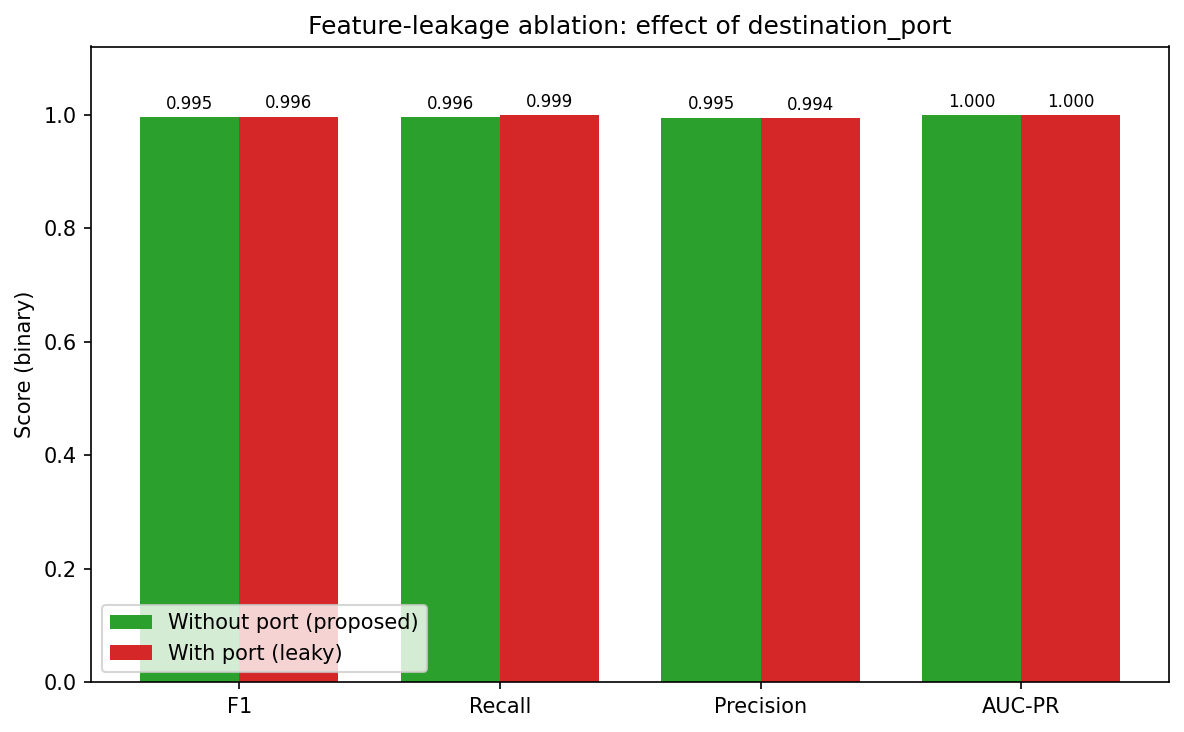
\includegraphics[width=0.7\textwidth]{leakage_ablation.png}%
  }{%
    \fbox{\parbox{0.66\textwidth}{\centering\vspace{1.2cm}\ph{Biểu đồ ablation rò rỉ --- chạy ml\_10\_leakage\_ablation.py}\vspace{1.2cm}}}%
  }
  \caption{Ảnh hưởng của đặc trưng rò rỉ \texttt{destination\_port} (Random Forest, nhị phân).}
  \label{fig:leakage-ablation}
\end{figure}

\subsection{So sánh bốn phương pháp giảm chiều}

\begin{figure}[htbp]
  \centering
  \IfFileExists{../../../results/ml_07_cross_method_comparison/f1_heatmap.png}{%
    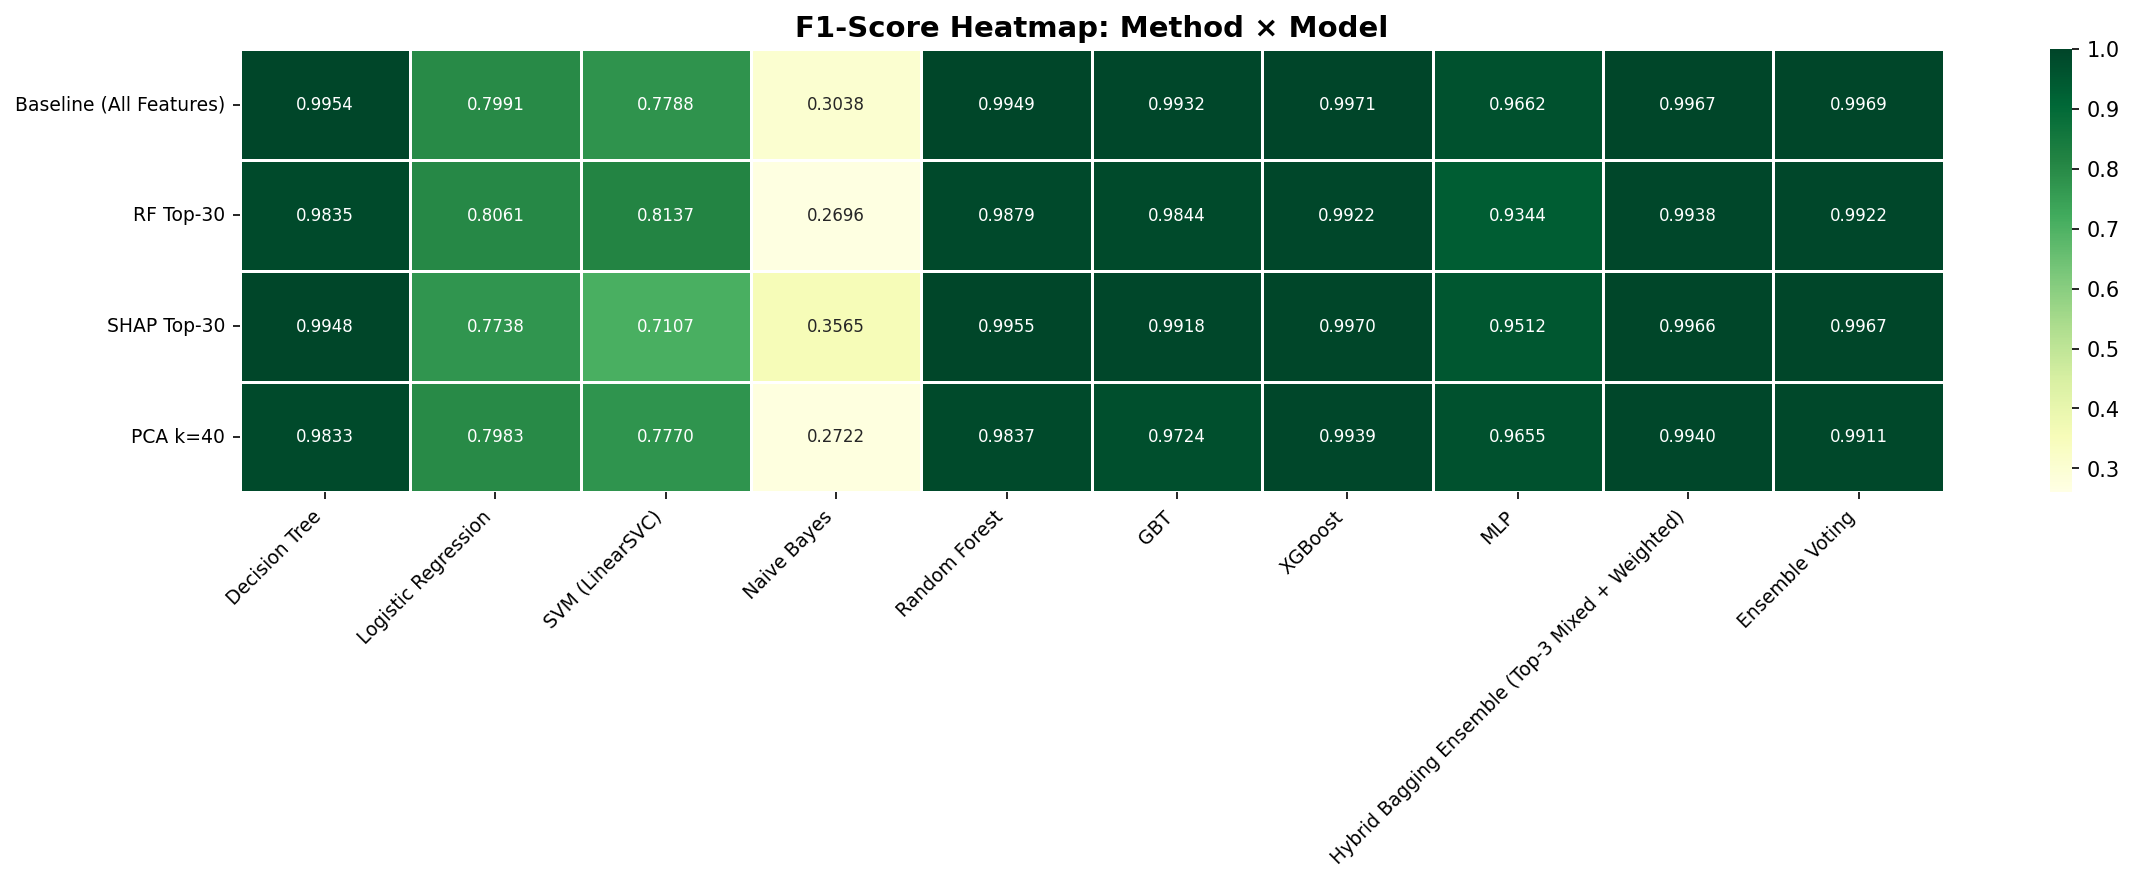
\includegraphics[width=0.92\textwidth]{f1_heatmap.png}%
  }{%
    \fbox{\parbox{0.88\textwidth}{\centering\vspace{1.5cm}\ph{Heatmap F1: phương pháp x thuật toán --- chạy thesis/collect\_results.sh}\vspace{1.5cm}}}%
  }
  \caption{Heatmap F1 theo phương pháp và thuật toán (nhị phân, đã loại cổng).}
  \label{fig:f1-heatmap}
\end{figure}

Bảng~\ref{tab:best-results} tóm tắt mô hình tốt nhất mỗi phương pháp. Lựa chọn đặc trưng (RF/SHAP Top-30) giữ hiệu năng gần baseline trong khi giảm $\approx$60\% số đặc trưng; PCA $k{=}40$ giảm chiều không giám sát với chi phí giải thích.

\begin{table}[htbp]
  \caption{Tóm tắt mô hình tốt nhất mỗi phương pháp (điền từ \texttt{cross\_method\_summary.csv}).}
  \label{tab:best-results}
  \centering
  \begin{tabular}{llcccc}
    \toprule
    Phương pháp & Mô hình & F1 & AUC-PR & Train (s) & Size (MB) \\
    \midrule
    Baseline & \ph{m1} & \ph{f1\_1} & \ph{pr\_1} & \ph{t\_1} & \ph{s\_1} \\
    RF Top-30 & \ph{m2} & \ph{f1\_2} & \ph{pr\_2} & \ph{t\_2} & \ph{s\_2} \\
    SHAP Top-30 & \ph{m3} & \ph{f1\_3} & \ph{pr\_3} & \ph{t\_3} & \ph{s\_3} \\
    PCA $k$=40 & \ph{m4} & \ph{f1\_4} & \ph{pr\_4} & \ph{t\_4} & \ph{s\_4} \\
    \bottomrule
  \end{tabular}
\end{table}

\begin{figure}[htbp]
  \centering
  \IfFileExists{../../../results/ml_07_cross_method_comparison/train_predict_time.png}{%
    \includegraphics[width=0.82\textwidth]{train_predict_time.png}%
  }{%
    \fbox{\parbox{0.78\textwidth}{\centering\vspace{1.2cm}\ph{Thời gian train/predict --- chạy ml\_07\_cross\_method\_comparison.py}\vspace{1.2cm}}}%
  }
  \caption{Thời gian huấn luyện và suy luận của mô hình tốt nhất mỗi phương pháp (đo trên cụm Spark Jetson).}
  \label{fig:timing}
\end{figure}

\subsection{Kiểm định thống kê (lấy mẫu lại ghép cặp)}

Bảng~\ref{tab:stat} báo cáo F1 trung bình $\pm$ CI 95\% (phân phối $t$) trên $N{=}6$ lần lấy mẫu lại cho hai phương pháp hàng đầu, kèm $p$-value permutation test ghép cặp. Kết luận: \ph{hai phương pháp tương đương ($p=$\,...) / khác biệt có ý nghĩa}.

\begin{table}[htbp]
  \caption{Ổn định đa lần lấy mẫu và kiểm định ghép cặp (điền từ \texttt{statistical\_validity\_multiseed.csv}).}
  \label{tab:stat}
  \centering
  \begin{tabular}{llcc}
    \toprule
    Phương pháp & Mô hình & F1 (mean $\pm$ CI95) & $p$ (ghép cặp) \\
    \midrule
    \ph{methodA} & \ph{modelA} & \ph{f1A} $\pm$ \ph{ciA} & \multirow{2}{*}{\ph{pval}} \\
    \ph{methodB} & \ph{modelB} & \ph{f1B} $\pm$ \ph{ciB} & \\
    \bottomrule
  \end{tabular}
\end{table}

\subsection{Robustness và đánh giá đa lớp}

Trên holdout tách rời, thứ hạng các phương pháp \ph{giữ nguyên/thay đổi}; chi tiết tại \texttt{robustness\_holdout\_summary.csv}. Đánh giá đa lớp (Hình~\ref{fig:cm}, Bảng~\ref{tab:perclass}) cho thấy các lớp đa số đạt recall cao, trong khi các lớp hiếm như \ph{lớp hiếm} có recall thấp hơn đáng kể (\ph{recall}) --- nơi lựa chọn đặc trưng tạo khác biệt rõ nhất.

\begin{figure}[htbp]
  \centering
  \IfFileExists{../../../results/ml_09_multiclass_eval/confusion_matrix.png}{%
    
\includegraphics[width=0.7\textwidth]{confusion_matrix.png}%
  }{%
    \fbox{\parbox{0.66\textwidth}{\centering\vspace{1.2cm}\ph{Ma trận nhầm lẫn đa lớp --- chạy ml\_09\_multiclass\_eval.py}\vspace{1.2cm}}}%
  }
  \caption{Ma trận nhầm lẫn đa lớp (chuẩn hoá theo hàng).}
  \label{fig:cm}
\end{figure}

\begin{table}[htbp]
  \caption{Precision/Recall/F1 theo lớp (trích từ \texttt{per\_class\_metrics.csv}).}
  \label{tab:perclass}
  \centering
  \begin{tabular}{lcccc}
    \toprule
    Lớp & Support & Precision & Recall & F1 \\
    \midrule
    \ph{lớp 1} & \ph{sup1} & \ph{p1} & \ph{r1} & \ph{cf1} \\
    \ph{lớp 2} & \ph{sup2} & \ph{p2} & \ph{r2} & \ph{cf2} \\
    \multicolumn{5}{c}{\ph{... các lớp còn lại; thêm dòng macro-F1 / weighted-F1}} \\
    \bottomrule
  \end{tabular}
\end{table}

\section{Thảo luận}
\label{sec:discuss}

\textbf{So sánh phương pháp.} Khi chênh lệch F1 giữa RF Top-30 và SHAP Top-30 nhỏ hơn biên dao động đa-lần-lấy-mẫu và $p>0{,}05$, ta kết luận hai phương pháp \emph{tương đương về mặt thống kê}; khi đó tiêu chí phụ (giải thích, kích thước, ổn định) quyết định lựa chọn triển khai. SHAP Top-30 cung cấp giải thích cục bộ nhất quán, lợi thế cho vận hành SOC.

\textbf{Cầu nối edge.} Giảm $\approx$60\% số đặc trưng trực tiếp giảm chi phí lắp ráp vector và bộ nhớ mô hình trên Jetson Orin Nano Super. Tiêu chí lựa chọn là \emph{edge-aware}: không chỉ F1 mà cả số đặc trưng, kích thước file và thời gian dự đoán. Benchmark latency/throughput trên Jetson trình bày trong công trình liên quan (SOICT 2026).

\textbf{Vì sao nhị phân chưa đủ.} Loại cổng và khử trùng kéo F1 nhị phân về mức thực tế, nhưng phân loại nhị phân vẫn dễ; đánh giá đa lớp mới phơi bày điểm yếu ở lớp tấn công hiếm và là thước đo phân biệt phương pháp đáng tin cậy hơn.

\section{Các mối đe doạ đến tính hợp lệ}
\label{sec:threats}

\textbf{Hợp lệ nội tại.} Xếp hạng RF/SHAP rút từ tập huấn luyện gốc và giữ cố định qua các lần lấy mẫu lại; nhất quán với thiết kế ``cấu hình a priori'' nhưng có thể tạo rò rỉ nhẹ ở phần ranking. Re-rank theo từng lần lấy mẫu sẽ chặt chẽ hơn nhưng tốn kém (đặc biệt SHAP); chúng tôi nêu rõ đánh đổi này. Ngoài ra, cân bằng lớp được áp đồng nhất cho bảy mô hình (Mục~\ref{sec:hparams}) nhưng \emph{không} cho MLP do Spark ML không hỗ trợ trọng số mẫu cho mô hình này; kết quả MLP vì vậy nên được đọc với lưu ý đó.

\textbf{Hợp lệ ngoại tại.} CICIDS2017 (2017) có thể không phản ánh lưu lượng hiện tại; cần kiểm chứng trên các bộ mới hơn (CSE-CIC-IDS2018, CIC-IoT). Phép chia ngẫu nhiên mặc định trộn thời gian; chế độ chia theo thời gian được hỗ trợ để đánh giá sát thực tế hơn.

\textbf{Hợp lệ thống kê.} Với $N{=}6$ lần lấy mẫu, permutation test vừa đủ để vượt ngưỡng $0{,}05$; tăng $N$, dùng corrected resampled $t$-test (Nadeau--Bengio) hoặc cross-validation lồng sẽ củng cố kết luận.

\section{Kết luận}
\label{sec:conclude}

Bài báo so sánh bốn chiến lược giảm chiều cho IDS trên Spark ML dưới một quy trình đánh giá chống rò rỉ và có kiểm định thống kê. Đóng góp cốt lõi không chỉ là ``phương pháp nào tốt nhất'' mà còn là \emph{cách đánh giá đáng tin cậy}: loại đặc trưng rò rỉ, khử trùng mức đặc trưng, robustness tách rời, kiểm định ghép cặp và đánh giá đa lớp. Hướng phát triển: mở rộng sang RoEduNet và CSE-CIC-IDS2018, tối ưu siêu tham số, và triển khai realtime trên edge.

\begin{credits}
\subsubsection{\ackname} Nghiên cứu thực hiện tại Trường Đại học Giao thông Vận tải (Phân hiệu TP.HCM) và Trường Đại học Công nghệ Thông tin, ĐHQG TP.HCM, trong khuôn khổ luận văn tốt nghiệp.
\subsubsection{\discintname} Các tác giả không có xung đột lợi ích.
\end{credits}

\bibliographystyle{../../latex/splncs04}
\bibliography{references,../../latex/related_work}

\end{document}
